
\usepackage[style=numeric,sorting=none]{biblatex}
\documentclass[]{article}
\usepackage[margin=1.25in,footskip=0.25in]{geometry}
\usepackage[english]{babel}
\usepackage[utf8]{inputenc}
\usepackage{amsmath}
\usepackage{graphicx}
\usepackage[colorinlistoftodos]{todonotes}
\usepackage{amssymb}
\usepackage{amsfonts}
\usepackage{hyperref}
\usepackage{algorithmicx}
\usepackage{algorithm}
\usepackage{algpseudocode}
\usepackage{framed,mdframed}
\usepackage{enumerate}
\usepackage{mathtools}
\usepackage{cite}
\usepackage{subcaption}
\usepackage{setspace}
\usepackage{amsthm}
\theoremstyle{definition}
\newtheorem{question}{Question}
\newtheorem{definition}{Definition}
\newtheorem{remark}{Remark}
\newtheorem{thm}{Theorem}[section]
\DeclareMathOperator{\E}{\mathbb{E}}
\newcommand{\Var}{\ensuremath{\mathsf{Var}}}
\newcommand{\Bin}{\ensuremath{\mathsf{Bin}}}

\usepackage[colorinlistoftodos,prependcaption,textsize-tiny]{todonotes}



\begin{document}



\title{Chapter 3 \hspace{1mm} Section 2}
\author{Mohamed Elmahy \\ Nowshin Sayara \\ Fariha Rashid }

\date{October 15, 2020}

\maketitle




\section{Introduction}


Algorithms can be beneficial when trying to perform a task or solve a problem.  Programmers need to choose the best-suited algorithm for any given program to optimize the performance better. There are many vital components to what makes an algorithm a good one. Notably, we look at the speed and number of steps involved. We can look at an algorithm's efficiency through asymptotic notations: Big O, Big Omega, and Big Theta. \\ \\
Big O describes an algorithm's worst-case by choosing a polynomial function's highest order, ignoring the constants. In contrast, Big Omega describes the best-case run time of an algorithm by selecting the polynomial function's lowest order, ignoring the constants. Finally, Big Theta describes both the best case and the worst-case run-time of an algorithm, which means the algorithm has to be both Big O and Big Omega simultaneously.

\section{Asymptotic Analysis}

\label{sec:examples}




\subsection{Importance}
Asymptotic analysis defines the run-time performance of an algorithm. Using asymptotic analysis, we can mathematically conclude the best case, average case, and worst case scenario of an algorithm.\\ \\
The time required by an algorithm falls under three types:
\begin{itemize}
\item Best Case - Minimum time required for program execution.
\item Average Case - Average time required for program execution.
\item Worst Case - Maximum time required for program execution.
\end{itemize}\\
\newpage
\section{Big-O Notation}
\subsection{Definition:}
We will need to let ${f}$  and ${g}$ be functions from ${Z \rightarrow R }$. We then say that ${f(x)}$ is ${O(g(x))}$. This is read as $"f(x)$ is big-oh of $g(x)."$ If there are constants ${C}$ and ${k}$ such that $|f(x)|\le C|g(x)|}$, whenever ${x > k}$.
To find a pair of witnesses, select a value of $k$ for which the size of ${|f(x)|}$ can be readily estimated when ${x>k}$ and then see whether we can use this estimate to find a value of ${C}$ for which ${|f(x)|\le C|g(x)|}$, \ whenever ${x > k}$.

\begin{figure}[h]
    \centering
    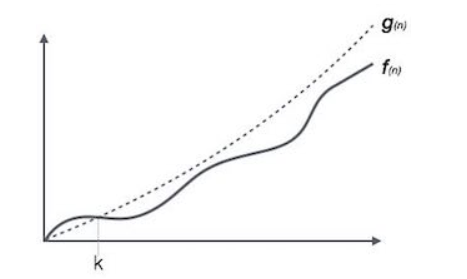
\includegraphics[width=10cm]{images/WUT.png}
    \caption{Big-O}
    \label{fig:WUT}
\end{figure}

\subsection{Importance of Big-O}
One of the advantages of using big-O notation is that we can estimate a function's growth without worrying about constant multipliers or smaller order terms. This means that, using big-O notation, we do not have to worry about the hardware and software used to implement an algorithm. The big-O notation is used extensively to estimate the number of operations an algorithm uses as its input grows.\ With the help of this notation, we can determine whether it is practical to use a particular algorithm to solve a problem as the input size increases.\\
\newpage
\subsection{Example}
\noindent \textbf{Question:}
Show that $7x^3$ is O$(x^2)$ \\
\begin{proof}
Assume that $7x^{^3}$ is O$(x^2)$, so by definition $\exists \hspace{2mm} c\ \ge\ 1}$, and ${k\ge0}$, such that 
\[{\frac{7x^3}{x^2}\le\frac{cx^2}{x^2}{,} \hspace{1mm} \forall x>k}\]
This implies
\[{7x \le c, \hspace{1mm} \forall x \ge k}\]
This is clearly false since $x$ is a variable and $C$ is a fixed constant.\ This means that $x$ will continue to grow to infinity. But clearly,
\[7x^2 \ is \  O(x^3)\]
\[x^2  \le x^3, \forall x \ge 1\]
Without a doubt, we know this is true.
\[\Rightarrow 7x^2\le7x^3{,} \hspace{1mm} \forall x \ge1\]
We multiply by 7 to get the original expression. By the previous equation, this is also true. So, ${C = 7}$ and ${k = 0}$ where ${x > k}$.
We choose k=0 because x is strictly greater than k. Therefore, 
\[7x^2\ \in\ O(x^3)\]
\end{proof}
\subsection{Example}
\textbf{Question:} Show that $n^2$ is not O$(n)$
\begin{proof} 
Assume that ${n^2 \in \ O(n)}$. Then by definition, ${ \exists \ C \ge1 {,} \ k \ge 0} \ such \ that \ {n^2 \ \le Cn}$. Which implies that
\[{n\ \le\ C, \ \forall n>k}\]
This is clearly false since $n$ grows infinitely. To show this,
take the limit as ${n \Rightarrow \infty}$ on both sides of the inequality.
\[\lim_{n\to\infty} n \ \le \lim_{n\to\infty} C}\]
Thus, ${\infty\le C}$, This is a contradiction, so ${\exists\ x{,} \ k}$ such that ${n^2\le\ Cn  {,}  \ \forall n>k$. Therefore, ${n^{2 }\notin\ O(n)$
\section{Big-O estimates for some important functions}
Polynomials can often be used to estimate the growth of functions. To do that we use Theorem 1 . It shows that the leading term of a polynomial dominates its growth by asserting that a polynomial of degree n or less is {\left(O(x^n\right)).}
\subsection{Theorem 1}
\begin{theorem}
${f(x)=a_nx^n+\dots+a_1x+a_0}$ where, $a_i$ are real numbers, then $f(x)$ is $O(x^n)$.\ This means that largest exponent in the polynomial equation defines the Big O.
\begin{proof}
Using triangle inequality, if $x>1$, we have, 
\begin{align*}
    |f(x)|& =|a_nx^n+a_{n-1}x^{n-1}+a_1x+a_0|\  \\ \\
    &  \le |a_n|x^n+|a_{n-1}|x^{n-1}+\dots+|a_1|x+|a_0| \\ \\
    & =x^n(\ |a_n|x^n+|a_{n-1}|x+\dots+|a_1|x^{n-1}+\frac{|a_0|\ }{x^n}) \\ \\
    & \le\ x^n(|a^n|+|a_{n-1}|+\dots+|a_1|+|a_0|) \\
\end{align*}
This shows that, ${|f(x)|\ \le\ Cx^n}$ where ${C=(|a_n|+|a_{n-1}|+\dots+|a_1|+|a_0|)}$ whenever ${x\ >\ 1}$.
Hence, the witnesses ${C=(|a_n|+|a_{n-1}|+\dots+|a_1|+|a_0|) }$ and ${k=1}$ show that ${f(x)} \ is \ {O(x^n)}$. \\ \\ 
\end{proof}
\end{theorem} \\
\subsection{Example}
\textbf{Question:}
Give big-O estimates for the factorial function and the logarithm of the factorial function, where the factorial function  ${f(n) = n!}$ \ is defined by ${n!=1\cdot 2\cdot 3\cdot \cdot \cdot n}$  \ whenever \ ${n}$ is a positive integer, and  ${0! = 1.}$
\begin{proof}
A big-O estimate for ${n!}$ can be obtained by noting that each term in the product does not exceed ${n}$. Hence, 
\[{n!=1\cdot2\cdot3\cdot\cdot\cdot n\ \le\ n\cdot n\cdot n\cdot\cdot\cdot n\ =\ n^n}\]
Each term can be upper bounded by $n$ since they are less than or equal to $n$.
The total number of inputs is n. Hence, we get $n^n$. 
This inequality shows that $n!$ is ${O(n^n)}$, taking  ${C=1}$  and  ${k=1}$ as witnesses. Taking logarithms of both sides of the inequality established ${n!}$, we obtain 
\[{\log\ n!\ \le\ \log\ n^n\ =\ n\log n}\]
This implies that ${\log\ n!} \ is \ {O(n\log n)}$. We choose ${C=1}$ and ${k=1}$ as witnesses.
\end{proof} 
\begin{figure}[h]
    \centering
    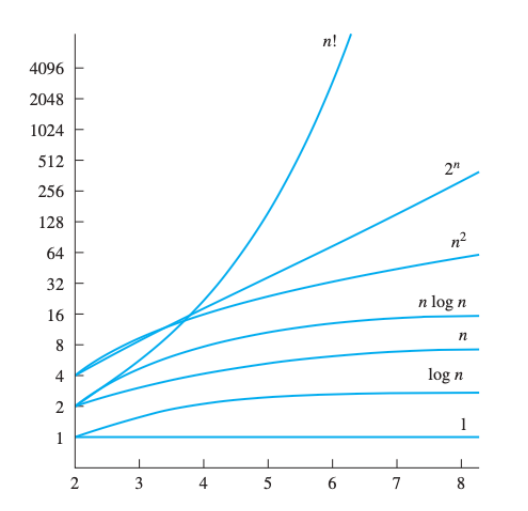
\includegraphics[width=8cm]{images/WUT2.png}
    \caption{A general hierarchy of functions, ordered by their growth complexity commonly used in big-O estimates: $1\ \le\log(n)\ \le\ n^c\ \le\ n^c\log(n)\ \le\ n^{c+\varepsilon}\le d^n\ \le n!\ \le n^n$ where \\ $c{,}\ \varepsilon\ \in(0{,}\infty)$ and $d\in(1{,}\infty).$}
    \label{fig:WUT2}
\end{figure}
\newpage 
\section{Useful things to know}
1) If ${d > c > 1}$, then  ${n^c \in O \left(n^d\right)$} but ${n^d\in O\left(n^c\right).$ This states that polynomials that have
a higher power can be a good upper bound for a general polynomial.
 \\ \\
2) Whenever ${b > 1}$ and ${c, d > 0}$, then  
${\left(\log_bn\right)^c =\log\binom{c}{b}\ n\in O\left(n^d)}$ but  ${n^d\notin O \left(\left(\log_bn\right)^c\right).$} This states that poly-logarithmic functions are less than polynomial functions. \\ \\
3) When ${c > b > 1}$, we have ${b^n\notin O\ \left(c^n\right)$} but ${c^n \notin O\left(b^n\right).}$ This states that the exponential function that has the bigger base is greater.\\ \\
4) If ${c > 1}$, we have that, ${n^c}$ is ${\ O\left(n!\ \right)}$ but ${n!}$ is not ${O\left(c^n).}$ This states that factorial functions grow faster than exponential functions.
\section{The growth of combinations of Functions}
A lot of algorithms use two or more separate sub-procedures.\ The number of steps used by a computer to solve a problem with the input of a specified size using such an algorithm is the sum of the number of steps used by these sub-procedures.\ To give a big-O estimate for the number of steps needed, it is necessary to find big-O estimates for the number of steps used by each sub-procedure and then combine these estimates.
\subsection{Theorem 2}
\begin{theorem}
Suppose that ${f_1(x)$ is $O(g_1(x))}$ and that ${f_2(x)$ is $O(g_2(x))}.$ Then ${( f_1 + f_2)(x)}$ is ${O(g(x))}$, where ${g(x) = (max(|g_1(x)| , \ |g_2(x)|)}$ for all ${x}.$
\end{theorem}
\subsection{Theorem 3}
\begin{theorem}
Suppose that ${f_1(x)}$ is ${O(g_1(x))}$ and ${f_2(x)}$ is ${O(g_2(x))}.$ Then ${(f_1f_2)(x)}$ is ${O(g_1(x)g_2(x))}.$ 
\end{theorem}
\subsection{Example} \\
\textbf{Question: }Give a big-O estimate for ${f(n)=3n\log(n!)+(n^2+3)\log n}$, where ${n}$ is a positive integer.
\begin{proof}
\begin{align*}
    f(n)&=3n\log(n!)+(n^2+3)\log n\\
    f_1(n)&=3n\log(n!)\\
    f_2(n)&=(n^2+3)\log n
\end{align*}
First, the product ${3n\log(n!)}$ will be estimated. From example 4.2, we know that $\log(n!)$ is $O(n\log n).$ Also, recall that $3n$ is $O(n)$ where $k=1$ and $C=3$. By using Theorem 3, we get
\[f_1(n)=(n^2+3)\log n \ \le \ O((n)(n\log n)) \ = \ O(n^2\log n)\]
Next, we find the Big-O of $(n^2+3)$ by upper bounding both terms.
\[n^2+3\le n^2+3n^2=4n^2\]
Therefore, $n^2+3$ is $O(n^2)$, where $k=1$ and $C=4.$ By Theorem 3 it follows that
\[f_2(n)=(n^2+3)\log n\ \le\ O((n^2)(\log n))\ =\ O(n^2\log n)\]
Use Theorem 2 to combine the two big-O estimates of $f_1(n)$ and $f_2(n)$ shows that 
\[f(n)\le O(\max(f_1{,} \ f_2))=O(\max(n^2\log n{,}\ n^2\log n))=O(n^2\log n)\]
Therefore, $f(n)$ is $O(n^2\log n)$.
\end{proof}
\section{Big-Omega Notation, \Omega}
Although big-O notation is used to describe the growth of a function, it does have some limitations to it.\ We have the upper bound when {f(x)  is  O(g(x))} in terms of {g(x)}, for the size of {f(x)} for large values of {x}, but we don't have the lower bound. This is why we use big-Omega notation. It gives us the lower bound, which is why it is used to describe the best case running time of an algorithm.
\subsection{Definition}
Let {f} and {g} be functions from the set of integers or the set of real numbers to the set of real numbers. We say that ${f(x)\  is\  \Omega\ (g(x))}$, which is read as $"{f (x)}$ is big-Omega of ${g(x)}"$. If there are constants {C} and {k} with $C>0$ such that
\[{\left|f(x)\right|\ \ge\ C\ \left|g(x)\right|}, \ whenever \ \ {x > k\]


\begin{equation*}
    }
\end{equation*}

\begin{figure}[h]
    \centering
    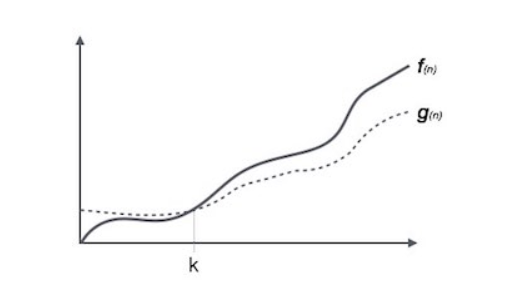
\includegraphics[width=11cm]{images/Omega.png}
    \caption{Omega Notation, \Omega}
    \label{fig:WUT}
\end{figure} \\
\subsection{Example} \\ 
\textbf{Question: }Show that ${f(x) = 8x^3+5x^2+7\ \in\ \Omega\ (x^3)}$
\begin{proof} We need to find a C value for which f(x) is greater.
\[{8x^3+5x^2+7\ \ge\ Cx^3}\]
Obviously
\[{8x^3+5x^2+7\ >\ 8x^{3}, \ \forall x\ge0}\]
Choose ${C=8}$ and ${k = 0}.$ Therefore, ${f(x)\ \in\ \Omega\ (g(x))}$.
\end{proof}
\section{Theta Notation, \theta}
When we want to give both an upper and a lower bound on the size of a function ${f(x)}$, relative to a reference function ${g(x)}$, we use big-theta ${(big- \theta)}$ notation. Big-theta is a stronger statement than big-O and big-omega because it is the most accurate and is true for all inputs.
\subsection{Definition}
Let ${f}$ and ${g}$ be functions. We say that
\[ {f(x)\  is\  \theta(g(x))} \ if \ {f(x) \in O(g(x))} \ and \ {f(x) \in \Omega\ (g(x)).}\]
\begin{equation*}
   
\end{equation*} 
\begin{figure}[h]
    \centering
    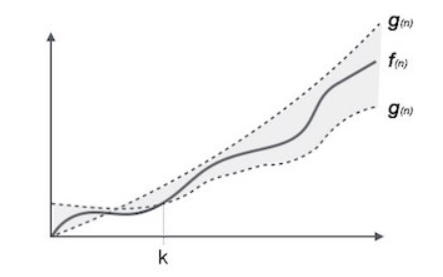
\includegraphics[width=10cm]{images/Theta.png}
    \caption{Theta notation, \theta}
    \label{fig:WUT}
\end{figure} 
\newpage
\subsection{Example} \\
\textbf{Question: }Show that  ${\sum_{i=1}^ni\ \in\theta\left(n^2\right)}$ \\ \\
\begin{proof}
First, we show that ${\sum_{i=1}^ni\ \in\ \Omega(n^2)}$
\begin{align*}
    1+2+\cdot\cdot\cdot+n\ \left &\ge\frac{n}{2}+(\frac{n}{2}+1)+(\frac{n}{2}+2)+\cdot\cdot\cdot+ n \\
    &\ge\frac{n}{2}+\frac{n}{2}+\cdot\cdot\cdot\cdot+\frac{n}{2}\\
    &\ge\frac{n}{2}(\frac{n}{2})
    =\frac{1}{4}n^{2\ }\in\ \Omega\ (n^2)
\end{align*}
First, we upper bound each term by $(\frac{n}{2})$ because it is halfway between 1 and n. Next, since we have \\ 
$(\frac{n}{2})$ terms in total, we multiply $(\frac{n}{2})$ with $(\frac{n}{2}).$ \\ \\
Next, we show that $\sum_{i=1}^ni\ \in \ O \left(n^2\right)}$
\begin{align*}
    \sum_{i=1}^ni\ &=\ 1+2+\cdot\cdot\cdot+n\\
    &\le n+n+\cdot\cdot\cdot+n \\
    &=n*n = n^2 \in O(n^2)
\end{align*}
We upper bound each term by n. Since the total inputs is n, we multiply n by n. We know that \\ \\ ${\sum_{i=1}^ni\ \in O\ \left(n^2\right)} \ and \ {\sum_{i=1}^ni\ \in\Omega\ \left(n^2\right)}$. Therefore, $ {\sum_{i=1}^ni\ \in\theta\ \left(n^2\right)}$
\end{proof}
\newpage
\section{Citation}
\begin{itemize}

1) Rosen, K. H. (2019). Discrete mathematics and its applications. New York, NY: McGraw-Hill.\\ \\
2) Roberts. (n.d.). Discrete Math: Big-O Examples and Theorems.\\
https://www.youtube.com/watch?v=ahTJ-TWCrrg&list=WL&index=3&t=573s&ab_channel=Dr.RobertsatGGC\\ \\ 
3) \ Data \ Structures - Asymptotic \ Analysis.\ (n.d.). 
Retrieved \ October \ 16, \ 2020, \ from \\ $https://www.tutorialspoint.com/data_structures_algorithms/asymptotic_analysis.htm$ 


\end{itemize}

\end{document}
